
\chapter{Verification with Dynamic Logic}
\label{cha:application}

We will now apply the general calculus as well as monad-specific extensions of
it to prove properties of monadic programs. These proofs will be fairly
detailed, which is so because of their being formal proofs. On the one hand this
provides rigorous evidence of their correctness, but on the other hand it 
definitely prompts for the employment of a \mbox{(semi-)} automatic proof assistant to
dispose of the necessity of doing the most trivial proof steps by hand. We begin
with some standard lemmas which are typical of dynamic logic.


\section{Basic Lemmas of Dynamic Logic}
\label{sec:basic-lemmas}

An important and quite natural fact is that one may prove formulae of the form
$\PDLBox{x\leteq p}{(\bigwedge\phi_i)}$ by proving each $\PDLBox{x\leteq p}{\phi_i}$ separately:
\begin{lem}
\label{thm:box-and-distrib}
 $\PDLBox{x\leteq p}(\phi \land \psi)\;$ if and only if $\;\PDLBox{x\leteq p}\phi \land
 \PDLBox{x\leteq p} \psi$
\end{lem}

\begin{proof}
\begin{itemize}
\item[``$\Rightarrow$''] We have $\phi \land \psi \Rightarrow \phi$, which is a tautology, so by (nec) and
  one-time application of modus ponens to (K1) we obtain $\PDLBox{x\leteq p}(\phi \land
  \psi) \Rightarrow \PDLBox{x\leteq p}\phi$.  Dually, we arrive at $\PDLBox{x\leteq p}(\phi \land \psi) \Rightarrow
  \PDLBox{x\leteq p}\psi$ when starting from $\phi \land \psi \Rightarrow \psi$. Taken together, the
  proposition is proved.

\item[``$\Leftarrow$''] Beginning with the tautology $\phi \Rightarrow (\psi \Rightarrow \phi \land \psi)$, by (nec) and
  two-time application of modus ponens to (K1) we arrive at $\PDLBox{x\leteq p}\phi
  \Rightarrow (\PDLBox{x\leteq p}\psi \Rightarrow \PDLBox{x\leteq p}(\phi \land \psi))$ which is tautologically
  equivalent to $\PDLBox{x\leteq p} \phi \land \PDLBox{x\leteq p} \psi \Rightarrow \PDLBox{x\leteq
    p}(\phi \land \psi)$.
\end{itemize}
\end{proof}

\begin{lem}[Regularity] \label{thm:regular}
  The following are valid rules of inference.
\[
  \NRule{reg\Box}{\forall x\bnd \phi \Rightarrow \psi}{\PDLBox{x\leteq p}{\phi} \Rightarrow \PDLBox{x\leteq p}{\psi}}
  \qquad
  \NRule{reg\Diamond}{\forall x\bnd \phi \Rightarrow \psi}{\PDLDmd{x\leteq p}{\phi} \Rightarrow \PDLDmd{x\leteq p}{\psi}}
\]
\end{lem}
\begin{proof}
  For $(reg\Box)$, assume $\forall x\bnd \phi \Rightarrow \psi$, apply necessitation to obtain
  $\PDLBox{x\leteq p}{\phi\Rightarrow\psi}$, from which the conclusion can be derived by modus
  ponens with (K1). The proof for rule $(reg\Diamond)$ is identical, except that (K2)
  has to be used in the final step.
\end{proof}


\begin{lem} \label{thm:wkbox-wkdmd}
  The following two rules that resemble modus ponens, only `inside'
  boxes and diamonds, are valid derived rules of inference. \\ 
\[
  \NRule{wk\Box}{[\xp]\phi \quad \forall x\bdot \phi \Rightarrow \psi}{[\xp] \psi}
  \qquad
  \NRule{wk\Diamond}{\langle\xp\rangle \phi \quad \forall x\bdot \phi \Rightarrow \psi }{\langle\xp\rangle \psi}
\]
\end{lem}
\begin{proof}
  Concerning  rule (wk$\Box$) we have to deduce the conclusion $[\xp]\psi$ under the
  assumptions $[\xp]\phi$ and $\forall x\bdot \phi \Rightarrow \psi$. By regularity, we immediately
  obtain $\PDLBox{x\leteq p}{\phi}  \Rightarrow \PDLBox{x\leteq p}{\psi}$, which provides the
  conclusion through an application of modus ponens with the assumption
  $\PDLBox{x\leteq p}{\phi}$. Once again, the proof of (wk$\Diamond$) is dual.
\end{proof}

The following lemmas, which can also be found in \cite{HarelKozen02}, show some
distributivity properties of the modal operators.  It should be pointed out that
the implications in the other directions are not valid (except for the first
lemma, where the reverse implication is axiom (K4)).

\begin{lem}
  $\xpdmd{\phi} \lor \xpdmd{\psi} \Rightarrow \xpdmd{\phi \lor \psi}$
\end{lem}
\begin{proof}
  This proof is rather typical and the same scheme will be applied to the
  following ones. First, we start with the tautology $\forall x\bnd \phi \Rightarrow \phi \lor \psi$;
  strictly speaking this is not a tautology due to the universal quantifier, but
  this formula can easily be obtained from the tautologous $\phi \Rightarrow \phi \lor \psi$ by
  universal generalisation, so we will talk of a formula as being a tautology
  even if it is the universal closure of one.

  By regularity we derive $\xpdmd{\phi} \Rightarrow \xpdmd{\phi \lor \psi}$, and we can also gain
  $\xpdmd{\psi} \Rightarrow \xpdmd{\phi \lor \psi}$ in a similar fashion. From these, twofold
  application of (mp) to the tautology scheme $(\Phi \Rightarrow \Theta) \Rightarrow (\Psi \Rightarrow \Theta) \Rightarrow (\Phi \lor \Psi \Rightarrow \Theta)$,
  where $\Phi = \xpdmd{\phi}, \Psi = \xpdmd{\psi}$ and $\Theta = \xpdmd{\phi \lor \psi}$, gives the
  desired result.
\end{proof}

\begin{lem}
  $\xpdmd{\phi \land \psi} \Rightarrow \xpdmd{\phi} \land \xpdmd{\psi}$
\end{lem}
\begin{proof}
  Here the tautology scheme is $(\Theta \Rightarrow \Phi) \Rightarrow (\Theta \Rightarrow \Psi) \Rightarrow \Theta  \Rightarrow \Phi  \land \Psi $ allowing us to
  separately prove $\xpdmd{\phi\land\psi} \Rightarrow \xpdmd{\phi}$ and $\xpdmd{\phi\land\psi} \Rightarrow \xpdmd{\psi}$ and
  then applying modus ponens twice. But these two formulae are directly provable
  from the obvious tautologies and application of rule (reg$\Diamond$).
\end{proof}

\begin{lem}
  \label{thm:more-distrib}
  The following implications are valid in the calculus. Proofs thereof are very
  similar to the previous ones and are therefore omitted.

  \begin{gather*}
      \xpdmd{\phi} \land \xpbox{\psi} \Rightarrow \xpdmd{\phi \land \psi} \\
      \xpbox{\phi} \lor \xpbox{\psi} \Rightarrow \xpbox{\phi \lor \psi}
  \end{gather*}
\end{lem}

\section{Axiomatising the Queue-Monad}
\label{sec:axiom-queue-monad}

Following the axiomatic approach to reasoning about a particular monad, the
first step is to characterise the monad by the signature of its basic operations
and a set of additional axioms. This is in contrast to the definitional approach
of \cite{IsabelleHOL}, where one  preferably defines the operations of the
monad and derives its properties as lemmas in the calculus on hand. The following
is a possible specification of a \emph{queue monad}, which comes with operations
to insert an element into the queue, to remove an element from the queue and
simultaneously return it as well as an operation for testing whether the queue
is empty. The signature of the operations is

\begin{flalign*}
&\mathbf{Operations} \\
&\enq : A \to Q\ 1 &&\\
&\deq : Q\ A\\
&\qmt : Q\ \Omega 
\end{flalign*}
where $A$ is a fixed type of queue elements, \IE $\enq$ and $\deq$ are not
polymorphic. A possible implementation of this monad is as a specific state
monad that maintains a list of elements of type $A$ as its state value.
\begin{flalign*}
&\textbf{Axioms} \\
&   \AssertDsef{\qmt}       && \text{(dsef-empty)}\\
&   \PDLDmd{\enq}\top                 && \text{(enq-term)}\\
&   \lnot \qmt \Rightarrow \PDLDmd{\deq}\top        && \text{(deq-term)}\\
&   \qmt \Rightarrow \PDLBox{\deq}\bot          && \text{(empty-deq)}\\
&   \PDLBox{\enq~z}\lnot \qmt        &&  \text{(non-empty)}\\
&   \qmt \Rightarrow \PDLBox{\enq~z; x \leteq \deq}(x=z \land \qmt) && \text{(enq-deq)}\\
&   \lnot \qmt \land \PDLBox{\enq~z; x \leteq \deq}\phi
   \iff  \lnot \qmt \land \PDLBox{x \leteq \deq; \enq~z}\phi && \text{(swap)}
\end{flalign*}


With these axioms we are able to establish some simple proofs about the queue
monad. For example, given an empty queue we can insert two items, fetch and
bind two items thereafter, and make a statement about the equality of items
inserted and fetched:

\begin{prop}
 $\qmt \Rightarrow [\enq~a; \enq~b; x \leteq \deq; y \leteq \deq](x=a \land y=b)$
\end{prop}

\begin{proof}
  We proceed in two steps, first asserting (a) $\qmt \Rightarrow [\enq~a; \enq~b; x \leteq
  \deq; y \leteq \deq](x=a)$, then (b) $\qmt \Rightarrow [\enq~a; \enq~b; x \leteq \deq;
  y \leteq \deq](y=b)$ and conclude by combining these two results by Lemma
  \ref{thm:box-and-distrib}

\begin{itemize}
% \setlength{\parskip}{1ex}
\item[(a)]
\[
\qmt \Rightarrow [\enq~a; x\leteq \deq](x=a) \land \qmt \qquad \text{by (enq-deq)}
\]
Noting that $x=a$ is stateless and thus applying (K3) and (seq$\Box$) we
obtain
\begin{equation}
\label{eq:seqeq1}
\qmt \Rightarrow [\enq~a; x\leteq\deq; \enq~b](x=a)
\end{equation}
By (swap) we have
\[
\lnot \qmt \Rightarrow [x\leteq \deq; \enq~b]\phi \Rightarrow [\enq~b; x\leteq\deq]\phi
\]
to which we apply (nec) and subsequently (K1) twice:
\[ \begin{split}
  [\enq~a]\lnot \qmt \Rightarrow 
   [\enq~a][x\leteq \deq; \enq~b]\phi \\
  \Rightarrow [\enq~a][\enq~b; x\leteq \deq]\phi
\end{split} \]

This can be simplified by (non-empty) and (seq$\Box$):
\begin{equation}
\label{eq:seqeq2}
[\enq~a; x\leteq \deq; \enq~b]\phi \Rightarrow [\enq~a; \enq~b; x\leteq \deq]\phi
\end{equation}
`Connecting' \eqref{eq:seqeq1} and \eqref{eq:seqeq2} by rule (wk$\Box$) provides
\[\qmt \Rightarrow [\enq~a; \enq~b; x\leteq \deq](x=a)\]
from which, finally, the proposition (a) can be derived by application of (K3)
and (seq$\Box$).

\item[(b)]

We have to show $\qmt \Rightarrow [\enq~a; \enq~b; x \leteq \deq; y \leteq
\deq](y=b)$ proceeding as follows and leaving applications of (seq$\Box$)
implicit. By (enq-deq) we respectively have
\[\begin{split}
\qmt \Rightarrow [\enq~a; x\leteq \deq]\qmt\\
\qmt \Rightarrow [\enq~b; y\leteq \deq](y=b)
\end{split}\]
These can be connected (with the help of rule wk$\Box$) to form
\begin{equation}
\label{eq:seqeq3}
\qmt \Rightarrow [\enq~a; x\leteq \deq; \enq~b; y\leteq \deq](y=b)
\end{equation}
Also, by (swap) we have
\[
\lnot \qmt \land [x\leteq \deq; \enq~b]\phi \Rightarrow [\enq~b; x\leteq \deq]\phi
\]
We once more apply (nec) and (K1) which brings us close to our goal:
\[ \begin{split}
[\enq~a]\lnot \qmt \Rightarrow [\enq~a;x\leteq \deq; \enq~b]\phi \Rightarrow \\
    [\enq~a; \enq~b; x\leteq \deq]\phi
\end{split} \]

The premiss can be disposed of by axiom (non-empty) so that we now
instantiate $\phi$ with $[y\leteq \deq](y=b)$ arriving at
\begin{equation}
\label{eq:seqeq4}
\begin{split}
[\enq~a;x\leteq \deq; \enq~b; y\leteq \deq](y=b) \Rightarrow \\
    [\enq~a; \enq~b; x\leteq \deq; y\leteq \deq](y=b)
\end{split}
\end{equation}
Now connect  \eqref{eq:seqeq3} and \eqref{eq:seqeq4} and we are done.

\end{itemize}
\end{proof}

We would now like to maintain an assertion concerning the termination of the
program sequence given above. This amounts to stating

\begin{prop}
$\langle \enq~a; \enq~b; \deq; \deq\rangle \top$
\end{prop}

Intuitively, one would say that any program sequence containing only $\enq$'s
and $\deq$'s in which every execution of $\deq$ is preceded by more $\enq$'s
than $\deq$'s should terminate unconditionally. Moreover, any program sequence
with the stated property and in which the total number of enq's exceeds the
number of deq's should enforce the queue not to be empty. This idea leads to the
following definition and theorem, from which the above proposition can be proved
with ease.

\begin{defn} In chance analogy to \cite{ClaessenHughes}, we say that a program
  sequence $p$ in the queue monad is \emph{well-formed} iff it is a non-empty
  sequence of programs $\enq~z_i$ or $x_i\leteq \deq$ in which every initial
  subsequence has the property of containing at least as many programs of the
  former type as of the latter type and in which $x_i \neq x_j$ for $i \neq j$.
\end{defn}

\begin{expl}
$(\enq~a; \enq~b; x \leteq \deq; y \leteq \deq)$ is a well-formed program
  sequence, whereas $(\enq~a; x\leteq \deq; y\leteq \deq)$ is not.
\end{expl}

\begin{thm}
\label{wf-empty}
 For every well-formed program sequence $p$ containing more enq's
than deq's one has $\PDLBox{p}\lnot \qmt$.
\end{thm}

\begin{proof} By induction on the number of occurrences of $\enq$.

In the base case $n=1$ there is only one possible program sequence, namely
$\enq~z$ for some $z$. Then, axiom (non-empty) gives us $[\enq~z]\lnot \qmt$.

In the inductive step, w.l.o.g. let $p$ consist of programs $\enq~z_i,\; 1\leq i\leq
n+1$ and $x_j\leteq \deq,\;1\leq j\leq m$ where necessarily $m\leq n$. We take a look at the final
occurrence of an $\enq$ and distinguish two possible cases:

(i) $p =( \ldots; \enq~z_{n+1})$, \IE the final $\enq$ appears at the end of the program
sequence. In this easier case, by repeated application of rule (nec) to $[\enq
z_{n+1}]\lnot \qmt$, which is an instance of axiom (non-empty), one obtains $[p]\lnot
\qmt$.

(ii) $p = (\ldots; \enq~z_{n+1}; x_{m-j}\leteq \deq; \ldots; x_{m}\leteq \deq)$. This can be proved by
induction on $j$. In the base case, where $j=0$, we have $p = (\ldots; \enq~z_{n+1};
x_{m}\leteq \deq)$ which means we can apply the `outer' induction hypothesis to the
$(\ldots)$ part providing $[\ldots]\lnot \qmt$. By (swap) we have 
\[
\lnot \qmt \Rightarrow [x_m\leteq \deq; \enq~z_{n+1}]\lnot \qmt \Rightarrow [\enq~z_{n+1}; x_m\leteq \deq]\lnot \qmt
\]
and
it thus suffices to show $[x_m\leteq \deq; \enq~z_{n+1}]\lnot \qmt$ which can be done by
applying rule (nec) to $[\enq~z_{n+1}]\lnot \qmt$, an instance of axiom (non-empty).

In the inductive step {\small ($j-1\to j,\;j>0$)},
$[\ldots; \enq~z_{n+1}; x_{m-j}\leteq \deq; \ldots; x_{m}\leteq \deq]\lnot \qmt$ has to be asserted. By the
outer inductive hypothesis we again have  $[\ldots]\lnot \qmt$, so by (swap) it suffices
to show 
\[
[\ldots; x_{m-j}\leteq \deq; \enq~z_{n+1}; x_{m-j+1}\leteq \deq; \ldots; x_{m}\leteq \deq]\lnot \qmt
\]
This is true due to the `inner' inductive hypothesis.
\end{proof}

Now we return to the deferred task of proving the termination of the above
program sequence, \IE we will prove $\langle \enq~a; \enq~b; \deq; \deq\rangle \top$.

\begin{proof}
By Lemma \ref{wf-empty} we have
\begin{equation}
\label{eq:seqterm1}
[\enq~a; \enq~b]\lnot \qmt \quad \mbox{and} \quad [\enq~a; \enq~ b; x\leteq \deq]\lnot \qmt 
\end{equation}
Now, $\langle \enq~a\rangle\top $ and $\langle \enq~b\rangle\top $ which is equivalent to $\top\Rightarrow\langle \enq~b\rangle\top$.
Thus, by rule (wk$\diamond$) and (seq$\diamond$): 
\begin{equation}
\label{eq:seqterm2}
\langle \enq~a; \enq~b\rangle \top 
\end{equation}
We prove $\langle \enq~a; \enq~b\rangle \lnot \qmt$ by application of (K2) to
\eqref{eq:seqterm1} and \eqref{eq:seqterm2}
once again noting that $\phi \iff  (\top \Rightarrow \phi)$.

In order to proceed to { $ \langle \enq~a; \enq~b; x\leteq \deq\rangle \top$} we apply rule
(wk$\diamond$) with the help of (deq-term). With the right-hand statement of \eqref{eq:seqterm1}
we can, in a very similar manner to the one just pointed out, assert $ \langle \enq~a;
\enq~b; x\leteq \deq\rangle \lnot \qmt$ in which we only need one further application of rule
(wk$\diamond$) and axiom (deq-term) to finish the proof.
\end{proof}

\Eat{One sees that with the help of Lemma \ref{wf-empty}, termination proofs of a series
of $\enq$'s and $\deq$'s are quite mechanical. One is thus inevitably attempted to
prove a more general statement about termination of these. This proof is left
out here for reasons that go beyond the scope of this scratch text XXX.}


% Recalling the axioms of the reference monad
%
% without new, since just one reference will be needed in the following

\section{Specification of a Reference Monad}
\label{sec:spec-ref-monad}

The algorithm of Section \ref{sec:bfs} will make use of a single reference to
store a result value in. Therefore we briefly review the axioms of a monad in
which such references are available. Further details can be found in
\cite{SchroederMossakowski:Hoare}. The reference monad $R$ is equipped with
operations for reading a reference $r : \op{Ref}\, A$, \IE a reference
containing a value of type $A$, and writing to it:
\begin{flalign*}
&\mathbf{Operations} \\
&\rd{\Arg} : \op{Ref}\,A \to R\,A &&\\
&(\Arg := \Arg) : \op{Ref}\,A \to A \to R\,1\\
\end{flalign*}

These operations should behave as expected, so that reading a value should be
\emph{dsef}, after writing to a reference, it should hold this value, and
writing to a  reference should not interfere with existing values of distinct
references.  
\begin{flalign*}
&\mathbf{Axioms} \\
&   \AssertDsef{\rd{r}}       && \text{(dsef-read)}\\
&   \PDLBox{r := x}{x = \rd{r}} && \text{(read-write)}\\
&   \PDLDmd{r := x}{\top} && \text{(write-term)}\\
&   (x = \rd{r}) \Rightarrow \PDLBox{s := y}{(x = \rd{r} \lor r = s)} && \text{(read-write-other)}
\end{flalign*}


% breadth first search as a monadic program
% proof of correctness
%
% Changelog:
% 2004-11-24 Created document, first attempt
%

\section{Correctness of a Breadth-First Search Algorithm}
\label{sec:bfs}

Breadth-first search is a commonly used, if memory intensive, technique for
finding an element in a tree satisfying a certain condition
(\cite{RussellNorvig}). Basically, this algorithm will be defined in the
previously axiomatised \emph{queue monad} $Q$, which is extended so as to include a
single \emph{reference of type A} which will be used to store elements of a tree
over $A$. Although in finite trees a proper search algorithm will always
terminate, its canonical definition requires the existence of an iteration
construct that resembles the while-loop of imperative languages. This iteration
construct is practically by definition not interpretable by a total function --
as is known it is the basic source of nontermination in simple imperative
languages. Therefore we will assume for this section that the underlying monad
allows the interpretation of arbitrary recursive definitions, \EG via fixed
point recursion on cpos. Although quite a far-reaching condition, there exist
monads that allow the interpretation of all operations used in this section.
Moreover we assume existence of a classical type of truth values $\Type{Bool}$
that is needed to interpret the \emph{if-then-else} construct in the
usual manner -- this requirement is of course not necessary if the underlying
logic is classical, so that $\Type{Bool}$ is the type of truth values anyway.
In this vein we can recursively define a while-loop in the following way:
\begin{flalign*}
  & \While : Q\ \Type{Bool} \to Q1 \to Q1 && \\
  & \While\ b\ p = \DoStmt{x\leteq b; \IfTerm{x}{\DoStmt{p; \While\ b\ p}}{\ret~\unit}}
\end{flalign*}

The algorithm whose correctness will be verified is then defined as 
{
\newcommand{\filla}{\hspace*{1cm}}
\newcommand{\fillaa}{\hspace*{2cm}}
\newcommand{\fillb}{\hspace*{0.5cm}}
\newcommand{\fillc}{\hspace*{0.25cm}}
\begin{flalign*}
  & \begin{array}{l}
    \op{bfs} : (A \to \Type{Bool}) \to \Type{Tree}\ A \to Q\ 1\\
    \op{bfs}\ p\ r = \DO\ \{\\
    \filla x := \inl~\unit;\\
    \filla \enq~r;\\
    \filla \While\ (\rd{x} = \inl~\unit \land \lnot\op{empty})\\
    \fillaa \DO\ \{\ t\leteq \deq;\\
    \fillaa \fillb \fillc \If\ (p~t)\ \Then\ x := \inr~t\\
    \fillaa \filla \fillc \Else\ \enqAll~(\chld~t)\\
    \fillaa \}\\
    \filla \}
    \end{array}
    & \mbox{}
\end{flalign*}
}\noindent
where $\enqAll$ is a primitive recursive function that simply inserts all given
elements into the queue:
\begin{flalign*}
  & \begin{array}{ll}
    \enqAll\ [] &= \ret~\unit\\
    \enqAll\ (x:xs) &= \DO\ \{\ \enq~x; \enqAll~xs\ \}
  \end{array} & \mbox{}
\end{flalign*}

To keep the discussion independent of a concrete implementation of a tree of
elements of type $A$, we simply assume its existence as well as some kind of
\emph{access function} $\op{chld}$ returning a list of a tree's child nodes.
$\inl$ and $\inr$ are the usual left and right injections for sum datatypes,
while $\unit$ is the single inhabitant of the unit datatype $1$, so that $x$ is
a reference over values of $1 + \Type{Tree}~A$. In what follows we will talk about a fixed, yet
arbitrary \emph{finite tree} $r$.

\begin{figure}
  \centering
  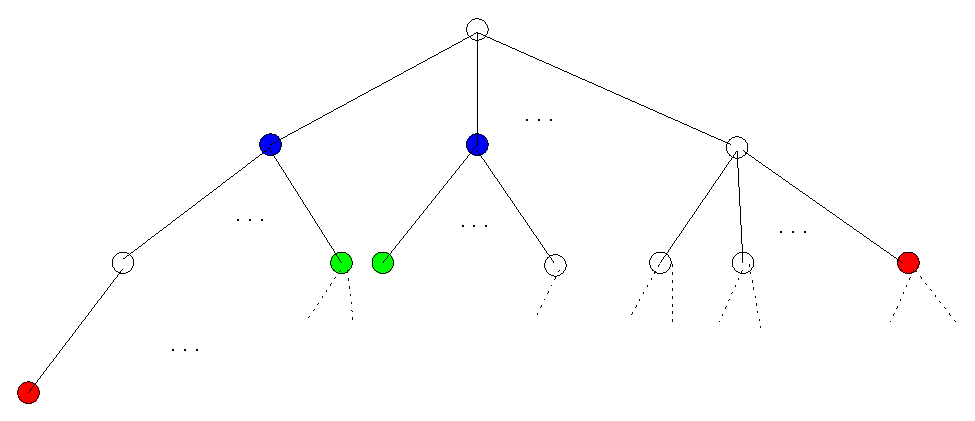
\includegraphics[width=0.7\textwidth]{tree}
  \caption{Graphical representation of a finitely branching tree; identically
    coloured nodes represent direct neighbours in the sense of $\prec_{1}$}
  \label{fig:finite-tree}
\end{figure}

The typical property of breadth-first search is that it `finds' the shallowest
node in the tree $r$ satisfying the property $p$, \IE in our case it assigns
this node to the reference $x$. Therefore, we impose an order $\prec_1$ on the
elements of the tree by defining a subtree $t_1$ to \emph{directly precede} a
subtree $t_2$ (written $t_1 \prec_1 t_2$) iff $t_1$ lies on the same level as $t_2$
does, \IE has the same depth, and the former is its direct left-hand neighbour,
or $t_1$ is the rightmost element in some level $n$ and $t_2$ is the leftmost
element in level $n+1$ (with respect to a graphical representation depicted in
Figure \ref{fig:finite-tree}). By taking the transitive closure $\prec$ of $\prec_1$
\[
t \prec t' \quad\defeq\quad \exists t_1\ldots t_n\bnd t \prec_1 t_1 \land t_1 \prec_1 t_2 \land \cdots \land  t_n \prec_1 t'
\]
we obtain a means to say that a subtree $t$ \emph{precedes} some other subtree
$t'$. From these definitions, it is clear that 
\[t_1 \prec t_2 \land \lnot \exists t \in r.\; t_1\prec t\prec t_2 \quad\text{iff}\quad t_1 \prec_1 t_2\]
To put it formally, our goal will then be  to prove
\[
  (\exists t \in r\bnd p\ t) \Rightarrow [\ibox{bfs p r}](\rd{x} = \inr~t_0 \land (p\ t_0) \land \forall t \in r\bnd p\ t \Rightarrow t = t_0 \lor t_0 \prec t)
\]
where, in the following we will be a bit sloppy about the value of $\rd{x}$ and
use $\rd{x}$ in place of the tree $t$ if $\rd{x} = \inr~t$, and say $\rd{x} =
\unit$ if actually $\rd{x} = \inl~\unit$. This will not lead to ambiguities,
since no tree is of the form $\unit$.
\begin{rem}
\label{rem-chld}
One has $t_1 \prec t_2 \Rightarrow \forall c_1\in\chld~t_1, c_2 \in \chld~t_2.\; c_1 \prec
c_2$, which is immediate from the definition of relation $\prec$. Also, for 
each tree $t$ where $\chld~t = [c_1,\ldots, c_n]$ it is clear that
$c_i \prec_{1} c_{i+1} \text{ for } 1\leq i<n$.
\end{rem}

% inq and relq
In order to reason about the contents of the current queue, we need two
additional monadic predicates $relq : (A \to A \to \Omega) \to Q\ \Omega$ and $inq : A \to Q\ \Omega $
which intuitively state that a given relation holds for adjacent elements in the
queue, respectively that an element is contained in the queue. One could define
these predicates by means of the iteration construct $\op{iter}$ for which an
inference rule exists (see \cite{SchroederMossakowski:PDL}). In this case,
however, the definitions as well as the proofs involving them become quite
unwieldy. We therefore take another approach and axiomatise one further
deterministically side-effect free operation $\get$, which lets us
\emph{look inside} the queue by returning a list of all elements in the queue.
We will use notation $(x:xs)$ for a list with head $x$ and tail list $xs$ as
well as $(xs\uparrow x)$ for a list with endmost element $x$ and initial part $xs$.

\begin{flalign*}
& \mathbf{Axioms}\\
& \AssertDsef{get} && \text{(dsef-get)} \\
& (\get = xs) \Rightarrow  \PDLBox{\enq~x}{(get = (xs\uparrow x))} && \text{(enq-app)} \\
& (\get = (x:xs)) \Rightarrow \PDLBox{y \leteq \deq}{(x = y \land \get = xs)} && \text{(deq-tl)} \\
& \qmt \iff (\get = []) && \text{empty-nil}
\end{flalign*}

An essential operation on queues we will need in our correctness proof is
$\op{last}$. With $\get$ available, this is just an abbreviation, assuming
there is a function $\op{lst}$ on lists that returns the last element in the list:

\[
(x = \last) \quad\defeq\quad x = (\op{lst}\ get)
\]

Obviously,
one has $(\get = xs\uparrow z) \Rightarrow (last = z)$.

\begin{defn}[$\relq$ and $\inq$]
\begin{eqnarray}
\label{eq:def-relq}
%\relq\  R &\defeq& \PDLBox{q\leteq\get}{(\forall i.\; 0\leq i<\op{len}\ q -1 \Rightarrow q^i R
%q^{i+1})} \\
\relq\  R &\defeq& \get = q \Rightarrow (\forall i.\; 0\leq i<\op{len}\ q -1 \Rightarrow q^i R q^{i+1}) \\
\label{eq:def-inq}
%\inq~ x &\defeq& \PDLBox{q \leteq \get}{(\exists i.\; 0\leq i<\op{len}\ q \land q^i = x)}
\inq~ x &\defeq& \get = q \Rightarrow (\exists i.\; 0\leq i<\op{len}\ q \land q^i = x)
\end{eqnarray}
Where $q^i$ denotes the $i$-th element of the list $q$, with the count
starting at zero.
\end{defn}

%% the loop invariant

The main problem, as often encountered in proofs involving a while-loop, is to
establish a loop invariant, \IE a condition that holds before the loop and is
re-established at each iteration of the loop.  Figure \ref{fig:inv} shows the
invariant for the while loop of the $\op{bfs}$ algorithm.  The first thing to
remain invariant is the in-queue relation $\relq~\prec_1$, as we will see. This
makes sure that all items in the tree are searched `in order'. Furthermore, if
$x$ has not been assigned a value, there are two cases: either the queue is
empty, in which case there is no element in the tree satisfying $p$ (which would
contradict the assumptions), or the queue is not empty and two conditions hold,
abbreviated as follows:
\begin{eqnarray}
\label{eq:def-nf}
NF(t) &\defeq& \forall t'\in r.\; t' \prec t \Rightarrow \lnot p\, t' \\
\label{eq:def-cin}
CIN(t) &\defeq& \forall c\in r.\; \inq~c \iff \exists t' \in r.\; c\in \chld~t' \land t' \prec t \prec c
\end{eqnarray}
$[t \leteq \deq]NF(t)$ states that for all elements preceding $t$ property $p$ does
not hold, and $[t\leteq \deq]CIN(t)$ states that the elements in the queue are
exactly the children of elements $t'$  preceding $t$, whose children are
preceded by $t$. Finally the case $\lnot (\rd{x}=\unit)$ must be considered, where it is said
that $p\, \rd{x}$ holds and all elements before $\rd{x}$ do not have property
$p$.

\begin{figure}
\begin{center}
\fbox{
  \begin{minipage}{0.8\textwidth}
    \centering
    \[
    \begin{array}{clcll}
      & \ibox{relq}\; \prec_1 &&& \\
      \land & \rd{x} = \unit &\Rightarrow& \lnot \qmt \land {} & [t \leteq \deq](NF(t) \land CIN(t)) \\
      &        &  &\multicolumn{2}{l}{ \lor (\qmt \land \lnot \exists t \in r\bnd p\ t)} \\
      \land & \lnot(\rd{x} = \unit) &\Rightarrow&\multicolumn{2}{l}{p\, \rd{x} \land \forall t \in r\bnd p\ t \Rightarrow \rd{x} = t
      \lor \rd{x} \prec t} \\
    \end{array}
    \]
  \end{minipage}
}
\end{center}
\caption[A loop invariant]{Loop invariant $INV$ for the proposed breadth-first search}
\label{fig:inv}
\end{figure}

\subsection{Basic Facts}
Before providing the proof, we note some basic facts we will use later on.
\begin{lem}
In a non-empty queue, $\enqAll$ and $\deq$ may be swapped:
\label{enqAll-deq}
\begin{eqnarray*}
&& \lnot \qmt \land [\enqAll~xs][t\leteq\deq]\varphi\;t \\
&\iff \quad& \lnot \qmt \land [t\leteq\deq][\enqAll~xs]\varphi\;t
\end{eqnarray*}
\end{lem}

\begin{proof}
By induction on the structure of $xs$. In the base case, $xs = []$, by
(dsef$\Box$) we have $[\ret~\unit]\varphi \iff \varphi$ and thus $[\enqAll~xs]\varphi \iff \varphi$
by the definition of $\enqAll$. So the base case is trivially true.

In the inductive step, let $xs = (y: ys)$, so we need to show
\begin{eqnarray*}
&& \lnot \qmt \land [\enq~y; \enqAll~ys][t\leteq\deq]\varphi\;t \\
&\iff \quad& \lnot \qmt \land [t\leteq\deq][\enq~y; \enqAll~ys]\varphi\;t
\end{eqnarray*}
By the inductive hypothesis, the left-hand part of the formula can be
equivalently 
reformulated as $\lnot \qmt\land [\enq~y][t\leteq\deq][\enqAll~ys]\varphi\;t$ and then, by axiom
(swap) this is equivalent to the right-hand side of the formula
\end{proof}


\begin{lem}
\label{thm:enq-relq}
Under the stated conditions, we can add an element into the queue without
losing property $\relq~R$:
\begin{eqnarray*}
\text{(i)} && \lnot \qmt \land \last\; R\;x \land \relq\  R \Rightarrow [\enq~x]\relq\  R \\
\text{(ii)} && \qmt \Rightarrow [\enq~x]\relq\  R
\end{eqnarray*}
\end{lem}

\begin{proof} 
  For (i), we reformulate $\lnot \qmt$ as $\get = xs\uparrow y$ (which indeed is an
  existential statement: there are some $xs$ and $y$ with this property), from
  which it follows that $\last\;R\;x$ is $yRx$ and $\relq\ R$ simplifies to 
  $\forall i\bnd 0\leq i<\op{len}\ xs \Rightarrow (xs\uparrow y)^iR(xs\uparrow y)^{i+1}$. The latter two formulae
  are stateless, such that together with axiom (get-app) one has
  \begin{equation*}\begin{split}
 \get = (xs\uparrow y) \land yRx \land \forall i\bnd 0\leq i<\op{len}\ xs \Rightarrow (xs\uparrow y)^iR(xs\uparrow y)^{i+1} \Rightarrow \\
  \PDLBox{\enq\ x}{\get = (xs\uparrow y\uparrow x) \land yRx \land \forall i\bnd 0\leq i<\op{len}\ xs \Rightarrow (xs\uparrow
    y)^iR(xs\uparrow y)^{i+1}}
  \end{split}
  \end{equation*}
where the formula in the scope of the box operator implies $\relq\ R$, which finishes
  the proof by an application of rule (wk$\Box$).


  Concerning (ii), the conclusion is obvious from the premiss and the definition
  of $\get$ and $\relq$.
\end{proof}


\begin{rem}
\label{rem:ext-enq-relq}
One can generalise Lemma \ref{thm:enq-relq} in the sense that it is also
possible to insert lists of items $[x_1,\ldots ,x_n]$ for all $n \in \mathbb{N}$ if
$x_i R x_{i+1}$ for $i \in \{1,\ldots,n-1 \}$ and $x_1$ may be enqueued without breaking
the relation $\relq\ R$.  The proof thereof proceeds by
structural induction on the to-be-inserted list.
\end{rem}

\begin{lem}
\label{thm:relq-deq}
If the relation $R$ holds in the queue, \IE $\relq\  R$, then after removing one
element, $R$ still holds: $\relq\  R \Rightarrow [x\leteq\deq]\relq\  R$. 
\end{lem}

\begin{proof}
For $\get = []$, the formula holds trivially, so assume $\get = (y: ys)$. From
the definition of $\relq$, we can deduce $\forall i.\; 0\leq i<len (y: ys) - 1 \Rightarrow
(y: ys)^iR(y: ys)^{(i+1)}$, so in particular $R$ holds for all adjacent
elements in $ys$. By (deq-tl) we obtain the desired result.
\end{proof}


\begin{lem}
\label{thm:enqAll-inq}
After inserting some elements $xs$ into the queue, for each $x\in xs$ we have
$\inq~x$. Put formally:
\[
[\enqAll~xs](\forall x\in xs\bnd \inq~x) \quad \text{for all lists $xs$}
\]
\end{lem}
\begin{proof}
  Since $\get$ is dsef and thus always defined, we always have $\get = ys$ for
  some list $ys$. Now as usual we proceed by induction on the structure of $xs$ and
  leave out the base case, where $\enqAll$ does nothing and there are no
  elements to make a statement about. So let $xs = (x':xs')$.  It then follows
  by (get-app) that $[\enq~x'](get = (ys \uparrow x'))$ and so $[\enq~x'](\inq~x')$. By
  the induction hypothesis we have
\[
[\enqAll~xs'](\forall x\in xs'\bnd \inq~x)
\]
and by application of (nec) we obtain
\[
[\enq~x'][\enqAll~xs'](\forall x\in xs'\bnd \inq~x)
\]
The missing ingredient for finishing the proof is
\[
\inq~x \Rightarrow [\enqAll~xs]\inq~x \quad \text{for all $x$ and $xs$}
\]
But this fact is again provable by induction on the mentioned $xs$ and follows
quite directly. Altogether we arrive at
\[
[\enq~x'][\enqAll~xs'](\forall x\in xs'\bnd \inq~x \land \inq~x')
\]
which actually is what we claimed, recalling that $(x':xs') = xs$
\end{proof}


%Actually, we do not have to axiomatise $\get$; it rather drops out of the
%previous axioms, if it is defined like follows.
%\begin{thm}
%\label{get-defn}
%Let
%\[
%\get\quad := (iter\; (\LambdaTerm{\Arg}{\lnot \qmt})\; (\LambdaTerm{z}{y \leteq \deq; ret (z\uparrow y)})\; [])
%\]
%In this case, the formulas \emph{enq-app}, \emph{deq-tl} and \emph{empty-nil}
%hold in a modified form accomodating the fact that $\get$, as defined here, is not dsef.

%XXX Not yet clear. No well-foundedness on the queue except empty, which we
%cannot say too much about.
%\end{thm}


%\begin{verbatim}
%deqAll :: Q a [a]
%deqAll = do if empty
%               then return []
%               else do x  <- deq
%                       xs <- deqAll
%                       return (x:xs)
%\end{verbatim}


%%%%%%%%%%%%%%%%%%%%
\begin{lem}
\label{deq-inq}
If the relation $\prec$ (or in fact any other strict partial order) holds in the
queue, then after removing an element $x$ from it, there is no element $y$ in
the queue with $x = y$
\[
\relq~\prec \quad\Rightarrow\quad [x \leteq \deq](\lnot \inq~x)
\]
\end{lem}

\begin{proof}
  We only need to consider the case where $\get = (y:ys)$. Assuming $\relq~\prec$
  amounts to saying that
\begin{equation}\label{eq:wasonestar}
\forall i.\; 0\leq i<len\ (y:ys) -1 \Rightarrow (y:ys)^i \prec (y:ys)^{i+1}
\end{equation}
holds. By (deq-tl), after dequeuing only the $ys$ remain in the queue:
\begin{equation}\label{eq:wastwostar}
\get = (y:ys) \Rightarrow [x \leteq \deq](\get = ys)
\end{equation}
Noting that $\prec$ is a transitive and irreflexive relation (\IE $\forall x\,y\,z\bnd x \prec
y \land y \prec z \Rightarrow x \prec z$ and $\forall x \bnd x \not\prec x$) we may by \eqref{eq:wasonestar}
infer that there is no $y'$ in $ys$ such that $y' = y$. But then, by
\eqref{eq:wastwostar}, we are already done: after dequeuing $x$, the $ys$
remain, in which there is no element equal to $x$.
\end{proof}

\begin{lem}
\label{inq-deq-eq}
Dequeuing an element does not affect existence of other elements inside the queue: 
\[
\inq~x \Rightarrow [y \leteq \deq](x = y \lor \inq~x)
\]
\end{lem}

\begin{proof}
  For $\get = []$, $\inq~x$ is obviously false for every $x$.  For $\get =
  [x_1,\ldots,x_n]$, assuming $\inq~x$ amounts to saying that there is an $x_i = x$
  for some $i,\; 1\leq i\leq n$. By (deq-tl) have $[y \leteq \deq](y = x_1 \land get =
  [x_2,\ldots,x_n]$ and thus for $x = x_1$ have $[y \leteq \deq](x = y)$ whereas for
  $x \neq x_1$ -- \IE $x = x_i$ for $1 < i \leq n$ -- have $[y \leteq \deq](\inq~x)$,
  so altogether $[y \leteq \deq](x = y \lor \inq~x)$ (cf. also Lemma
  \ref{thm:more-distrib}).
\end{proof}

\subsection{Auxiliary Rules}
\label{sec:auxiliary-rules}

In merging the specifications of the queue monad and the reference monad, a
typical frame-problem arises: The question \emph{`what remains the same in a
  changing world?'} can be instantiated here as \emph{`what happens to
  references if we modify the queue?'} The answer will certainly be
\emph{`nothing'}, which we formalise as follows.
\begin{equation}
\label{eq:frame1}
(x = \rd{r}) \Rightarrow [\mathit{qop}](x = \rd{r}) \quad\text{for }\mathit{qop} \in \{\deq, \enq, \qmt \} 
\end{equation}
The simplest way to answer the converse question \emph{`what happens to the queue
if we modify a reference?'}  is by relating $\get$ to reference writing:
\begin{equation}
\label{eq:frame2}
(\get = xs) \Rightarrow [r := x](\get = xs)
\end{equation}
Reference to one of these axioms will be indicated by (frame).

In \cite{SchroederMossakowski:PDL} a Hoare calculus for total correctness has been
developed, in which Hoare rules such as
\[
\text{\bf (seq)}\quad
\begin{array}{@{}c@{}}
[\varphi]\overline{x} \leteq \overline{p}[\psi] \\
{}[\psi]\overline{y} \leteq \overline{q}[\chi] \\\hline
{}[\varphi]\overline{x} \leteq \overline{p}; \overline{y} \leteq \overline{q}[\chi]
\end{array}
\]
appear. It has been said in Section \ref{sec:hoare-calculi} that a Hoare rule
$[\varphi]\overline{x} \leteq \overline{p}[\psi]$ is meant to be interpreted as $\varphi \Rightarrow
(\langle\overline{x} \leteq \overline{p}\rangle\top \land [\overline{x} \leteq \overline{p}]\psi)$. In
this way, partial correctness as well as termination of a program sequence
$\overline{p}$ and thus total correctness are concisely captured.

Because we are working with formulae of dynamic logic and do not want to switch
into the Hoare calculus, yet we would like to use the results of the latter, we
simply translate some Hoare rules of \cite{SchroederMossakowski:PDL} 
back into rules for dynamic logic.

\begin{eqnarray*}
\NRule{dsef1}{\text{p dsef}}{\varphi \Rightarrow [p]\varphi}
\qquad
\NRule{if}{\begin{array}{@{}c@{}}
             \text{b dsef}\\
             \varphi \land b \Rightarrow [x \leteq p]\psi\\
             \varphi \land \lnot b \Rightarrow [x \leteq q]\psi
           \end{array}}
           {\varphi \Rightarrow [x \leteq \IfTerm{b}{p}{q}]\psi}
\\
% \\
% \text{\bf (dsef2)}\quad
% \frac{\text{p dsef}}{[x \leteq p](x = p)}
% \qquad
% 
% \qquad
% \text{\bf (seq)}\quad
% \begin{array}{@{}c@{}}
% \varphi \Rightarrow [\overline{x} \leteq \overline{p}]\psi \\
% {}\psi \Rightarrow [\overline{y} \leteq \overline{q}]\chi \\\hline
% {}\varphi \Rightarrow [\overline{x} \leteq \overline{p}; \overline{y} \leteq \overline{q}]\chi
% \end{array}
\NRule{while}{\begin{array}{@{}c@{}}
                t : DB\\
                \Arg < \Arg : B \times B \to \Omega \text{ is well-founded}\\
                \varphi \land b \Rightarrow \PDLDmd{p}{\top}\\
                (\varphi \land b \land t =_B z) \Rightarrow [p](\varphi \land t < z) \end{array}}
     {\varphi \Rightarrow \PDLBox{\WhileTerm{b}{p}}{(\varphi \land \lnot b)} \land \PDLDmd{\WhileTerm{b}{p}}{\top}}
\end{eqnarray*}

In rule (while) termination is ensured by letting the term $t$ decrease strictly
in every iteration. Since $<$ is well-founded, it is impossible for the final
premiss to be true infinitely often. The so called \emph{ghost variable} $z : B$
does not appear within the program and simply serves the purpose of relating the
value of $t$ before and after execution of $p$. In particular, $t$ is not equal
to $z$ as a computation, but rather its value equals $z$.

Now we are equipped with all we
need to prove total correctness of the program $\op{bfs}$, in particular -- as
can be seen from the rule for while -- termination of the while-loop.

%%%%%%%%%%%%%%%%%%%%%%%%%%%%%%%%%%%%%%%%%%%%%%%%%%
% The proof
\subsection{Proof of Total Correctness}

In what follows, we try not to be too formalistic and therefore make reference
to common laws such as transitivity of equivalence or other obvious validities
without proving them for each separate instance.  We further assume that the
underlying formalism is classical, \IE we allow reasoning by case distinction
over some formula $\phi \lor \lnot \phi$. In a Hilbert-style calculus with essentially only
modus ponens available as an inference rule, methods such as proof by
contradiction are to be conceived as first proving $\lnot P \Rightarrow \False$ and then
applying (mp) to the tautologous $(\lnot P \Rightarrow \False) \Rightarrow P$. Likewise, substitutivity
of equivalence makes use of the tautology scheme $(P \iff Q) \Rightarrow R[P/x] \Rightarrow R[Q/x]$.

It will now first be established that $INV$, the loop invariant, holds before the while
loop, \IE with $PRE \defeq \exists t \in r\bnd p\ t$ (a stateless formula) we show 
\begin{equation}
\label{eq:est-inv}
PRE \land \qmt \Rightarrow [x := \unit ; \enq~r](INV)
\end{equation}

\begin{subequations}
By (read-write) and (frame)
\begin{equation}
\label{eq:est01}
[x := \unit; \enq~r](\rd{x} = \unit) 
\end{equation}
From the definition of $\relq$ we can infer
\begin{equation}
\qmt \Rightarrow [\enq~r](\relq~\prec)
\end{equation}
which by (frame) can be extended to
\begin{equation}
\label{eq:est02}
\qmt \Rightarrow [x := \unit; \enq~r](\relq~\prec) 
\end{equation}
Again with (frame), (enq-deq) gives us
\begin{equation}
\label{eq:est03}
\qmt \Rightarrow [x:= \unit; \enq~r][t \leteq deq](r = t \land \qmt)
\end{equation}
\end{subequations}

Now from $r = t$ we can deduce $NF(t)$, because there simply is no element $t' \prec
r$ in $r$. Similarly, we infer $CIN(t)$ because $\inq~c$ is false for every
element in $r$ and again there is no element $t' \prec r$, so the equivalence in
$CIN$ holds.  Combining (\ref{eq:est01}), (\ref{eq:est02}) and (\ref{eq:est03})
we obtain the desired result.

\paragraph{The while Rule}
The next step is to gather the premisses of the (while) rule as stated above to
draw the conclusion of selfsame. The premiss $INV \land \rd{x} = \unit \land \lnot \qmt \Rightarrow
\PDLDmd{\op{body}}{\top}$ asserting termination of the loop body $\op{body}$ is
quite obvious, since the only source of nontermination is the $\deq$-operation,
which will however only be executed if the queue is not empty. The formalisation
of this argument can be conducted along the lines of the following proof of the
most integral part:
\begin{equation}
\label{eq:prem-while}
\begin{array}{l}
INV \land \rd{x} = \unit \land \lnot \qmt \land vol = z \Rightarrow \\
 \qquad 
   [t \leteq \deq; \mathrm{if}\; p\ t\; \mathrm{then}\; x := inl\ t \;
   \mathrm{else}\; \enqAll~\chld
t](INV \land vol < z)
\end{array}
\end{equation}
where we introduce the termination measure $vol$ which computes the total number
of elements reachable from any subtree contained in the queue. Employing the
list functions $\op{sum} : [Nat] \to Nat$ and $\op{map} : (A \to B) \to [A] \to [B]$ --
whose definitions are straightforward and can be found, \EG, in the Haskell
Prelude -- it might be defined like this:
{
\newcommand{\filla}{\hspace*{1cm}}
\newcommand{\fillb}{\hspace*{0.75cm}}
\begin{flalign*}
  & \begin{array}{l}
    \op{vol} : Q\ \Type{Nat}\\
    \op{vol} = \DO\ \{\ q\leteq \get;\\
    \filla \fillb      \ret~\op{sum}~(\op{map}\ \op{volume}~q)\\
    \fillb \mathrm{where}\ \op{volume} : \Type{Tree}\ A \to \Type{Nat}\\
    \filla \fillb \op{volume}\ t = 1 + \op{sum}\ (\op{map}\ \op{volume}\ (\chld~t))
  \end{array} & \mbox{}
\end{flalign*}
}
\noindent
The intuition behind this approach is that the overall volume of the queue must
strictly decrease after dequeuing some subtree $t$ and enqueuing its children,
because the volume of $t$ is defined to be by 1 larger than the sum of volumes
of its children. $\op{vol}$ is a dsef operation since it is composed solely of
dsef operations (it has been shown in \Isabelle that dsef programs are stable
under composition).

% tomorrow never dies
We note the following equivalence which we shall use for simplification purposes
and whose right-hand part we will denote by $SI$.
\begin{eqnarray}
\label{eq:inv-equiv}
&& INV \land \rd{x} = \unit \land \lnot \qmt \\
&\iff& {\relq~\prec_1} \land \lnot \qmt \land [t \leteq \deq](NF(t) \land CIN(t)) \land \rd{x} = \unit 
\nonumber
\end{eqnarray}

By Lemma \ref{thm:relq-deq} we have
\[
SI \Rightarrow [t \leteq \deq](\relq~{\prec}_1)
\]
so by (frame) $\relq$ still holds after assignment to $x$:
\begin{equation}
\label{eq:then-part1}
SI \Rightarrow [t \leteq \deq][x := t](\relq~{\prec}_1)
\end{equation}

\paragraph{Then-branch} 
Working our way through the
then-branch of the loop body, we also need the next statement. This is
obtained from (read-write) and the fact that $NF$ and $p\; t$ are stateless.
\begin{equation}
\label{eq:then-part2}
NF(t) \land p\;t \Rightarrow [x := t](\rd{x} = t \land p\;\rd{x} \land NF(t))
\end{equation}
Now, $NF(t) \land p\;\rd{x} \land \rd{x} = t$, \IE that all elements in the tree smaller
than $t$ do not have property $p$, but $t$ and therefore $\rd{x}$ does, can be
reformulated as $p\;\rd{x} \land \forall t\in r\bnd p\;t \Rightarrow \rd{x} = t \lor \rd{x} \prec t$. 
% Regarding
% the decrease in volume, one has $\lnot \qmt \iff get = (x:xs)$ for some list $(x:xs)$
% and thus 
% \begin{equation}
% SI \land get = (x:xs) \land vol = z \Rightarrow [x:= t]
% \end{equation}


In combining
\eqref{eq:then-part1} and \eqref{eq:then-part2} we obtain the following, where
the formula in the scope of the  $[x := t]$ box is in fact stronger than $INV$
\begin{equation}
\label{eq:prem-then}
\begin{array}{l@{\quad}l}
& \relq~{\prec}_1 \land NF(t) \land p\;t \\
 \Rightarrow& 
   [x := t](\rd{x} = t \land p\;\rd{x} \land \relq~{\prec}_1\\
&\qquad {} \land (\forall t'\in r\bnd p\;t\Rightarrow\rd{x} = t' \lor \rd{x} \prec t')
\end{array}
\end{equation}

\paragraph{Else-branch}
Because all ingredients needed for the then-part are now assembled, we turn our
eyes to the else-part, which actually is the harder one. `Inside' the $[t \leteq
\deq]$ box of \eqref{eq:prem-while}
we have $CIN(t) \land NF(t) \land \relq~{\prec}_1 \land \rd{x} =  \unit$. We will, in accordance with the if-rule,
furthermore assume $\lnot p\;t$ and prove the following, in which again the formula
inside the $[\enqAll~(\chld~t)]$ box implies $INV$
\begin{equation}
\label{eq:prem-else}
\begin{array}{l@{\quad}l}
&  CIN(t) \land NF(t) \land \relq~{\prec}_1 \land \lnot p\;t \land \rd{x} =  \unit \\
\Rightarrow & [\enqAll~(\chld~t)](\relq~{\prec}_1 \land \rd{x} =  \unit   \\
&  \quad {}\land (\lnot \qmt \land [t' \leteq \deq](NF(t') \land CIN(t')) \\
& \qquad  {}\lor (\qmt \land \lnot \exists t''\in r\bnd p\;t'')))
\end{array}
\end{equation}
This can by Lemma \ref{thm:box-and-distrib} be done in three steps, each asserting
the truth of the above formula reduced to one of the three conjunct clauses in
the scope of the enqAll box.

\paragraph{Part i}
\[
% CIN(t) \land NF(t) \land \relq~{\prec}_1 \land \lnot p\;t \land 
\rd{x} = \unit \quad \Rightarrow 
\quad [\enqAll~(\chld~t)]\;(\rd{x} =  \unit )
\]
Now this is an obvious generalisation of one of the (frame) axioms.

\paragraph{Part ii}
\begin{align*}
  & CIN(t) \land NF(t) \land \relq~{\prec}_1 \land \lnot p\;t \land \rd{x} = 
  \unit \\
  \Rightarrow\quad& [\enqAll~(\chld~t)]\,(\relq~{\prec}_1)
\end{align*}
This formula asserts that we may enqueue $t$'s children without destroying the
relation $\relq~\prec_1$ inside the queue. For $\chld\ t = []$ we must then prove
\[ \ldots \land \relq~{\prec}_1 \land \ldots \Rightarrow \PDLBox{\ret~\unit}{\relq~{\prec}_1}\]
 which essentially is given by
(ret$\Box$). So let $\chld\ t = (x:xs)$.  Then by Remark \ref{rem:ext-enq-relq} all
children may be inserted through $\enqAll$ without invalidating $\relq~{\prec}_1$ if
$x$ may be enqueued through $\enq$. For $\qmt$ this is clearly true, so
consequently we'll add the premiss $\lnot \qmt$. Then $CIN(t)$ tells us $\inq~c$
holds for exactly all the child elements $c$ of predecessors of $t$. Thus $\last
\prec x$ certainly holds (cf. Remark \ref{rem-chld}). Because $\lnot \exists a\in r\bnd \last \prec
a \prec x$, even $\last \prec_1 x$ is true, providing all the premisses of Lemma
\ref{thm:enq-relq} and letting us draw the desired conclusion. $\lnot \exists a\in r\bnd
\last \prec a \prec x$ can be shown by contradiction: assume $\exists a\in r\bnd \last \prec a \prec x$;
Then it directly follows that there is $t''$ such that $a \in \chld~t''$ and $t''
\prec t$ ($t'' = t$ cannot be the case since $a \prec x$, and for the same reason $t \prec
t''$ neither). But then, because of $CIN(t)$, $\inq~a$ holds, which together
with $\last \prec a$ violates the given premiss $\relq~{\prec}_1$. We conclude that
part ii is true.

\paragraph{Part iii}
\begin{align*}
  & CIN(t) \land NF(t) \land \relq~{\prec}_1 \land \lnot p\;t \land \rd{x} =  \unit\\
 \Rightarrow\quad & [\enqAll~(\chld~t)]\,(\lnot \qmt \land [t' \leteq \deq](NF(t') \land CIN(t')) \\
 & \quad  {}\lor (\qmt \land \lnot \exists t''\in r\bnd p\;t''))
\end{align*}
This part makes sure that after inserting $t$'s child elements we either have seen
each element in the tree and none satisfies $p$, or there are elements left and
after dequeuing another element $t'$ all its predecessors don't have property
$p$ and the elements remaining in the queue are exactly the children of
predecessors of $t'$, which themselves are succeeding $t'$.

We proceed by case distinction over $\qmt \lor\lnot \qmt$. We have 
\[ \qmt \Rightarrow [\enqAll~(\chld~t)]\;\qmt \quad\text{iff}\quad \chld~t = []
\]
 But in this case, \IE when $\qmt$ holds in the box, $t$
must be the final element in the tree $r$ since all children of predecessors
would otherwise be in the queue (by $CIN$). Extend $NF(t)$ and $\lnot p\;t$ to $\lnot \exists
t''\in r\bnd p\;t''$ and obtain $[\enqAll~(\chld~t)](\qmt \land \lnot \exists t''\in r\bnd
p\;t'')$ making the conclusion of part (iii) true. For $\chld~t = (x:xs)$
one has $\qmt \Rightarrow [\enqAll~(\chld~t)](\lnot \qmt)$. Here, $t \prec_1 x$ must hold, \IE
t's first child element is its direct successor, because no element before $t$
has child elements that are in the queue by $CIN(t) \land \qmt$.  Now
\[
[\enq~x; \enqAll~xs][t' \leteq \deq](NF(t') \land CIN(t')))
\]
is by Lemma \ref{enqAll-deq} equivalent to 
\[
[\enq~x; t' \leteq \deq][\enqAll~xs](NF(t') \land CIN(t'))
\]
and because of (enq-deq) one has:
\[
\qmt \Rightarrow [\enq~x; t' \leteq \deq; \enqAll\ xs](x = t')
\]
So it suffices to prove the implication
\[ 
\ldots \Rightarrow [\enq~x; t'\leteq\deq][\enqAll~xs](CIN(t') \land NF(t'))
\]
where $\ldots$ denotes the premisses $\lnot p\,t$, $t {\prec}_1 x$, $CIN(t)$, $NF(t)$ and
$\qmt$.

The $NF$ part is fairly easy to see: one certainly has $NF(t) \land t {\prec}_1 t' \land \lnot
p\,t$ inside the box, which implies $NF(t')$, where $t'$ replaced $x$ due to
their being equal.  $CIN(t')$, which decodes into $CIN(t') \defeq
\forall c\in r.\; \inq~c \iff \exists t'' \in r.\; c\in \chld~t'' \land t'' \prec t' \prec c$, is true due to the
fact that exactly the $xs$ are in the queue, and for each $x' \in xs$ we have $x'
{\prec} x$. That finishes the case where $\qmt$ is true.

Now for the case where $\lnot \qmt$ is taken as a premiss and -- to restate the
other ones -- $CIN(t)$, $NF(t)$, $\relq~\prec_1$ and $\lnot p\,t$. Obviously one then has
$\ldots \Rightarrow [\enqAll~(\chld~t)](\lnot \qmt)$, so it remains to be proved that
\[
\ldots \Rightarrow [\enqAll~(\chld~t)][t' \leteq \deq](NF(t') \land CIN(t'))
\]
or, equivalently and quite similar to the case above we can show
\[
\ldots \Rightarrow [t' \leteq \deq][\enqAll~(\chld~t)](NF(t') \land CIN(t'))
\]
For $NF(t')$ alone, this can be done if $\ldots \Rightarrow [t' \leteq \deq](t {\prec}_1 t')$ can be shown,
because unlike $CIN(t')$, $NF(t')$ is indeed a stateless formula about a
property of the tree $r$ and not about the monadic queue. Hence $NF(t') \Rightarrow
[\enqAll~(\chld~t)](NF(t'))$ by (K3$\Box$). For
the same reason, however, $NF(t)$ holds after execution of $\deq$: $NF(t) \Rightarrow [t'
\leteq \deq](NF(t))$ so that at least for $NF(t')$ the proof goes through: we have
\begin{equation}
\label{eq:deq-nf}
\ldots \Rightarrow [t' \leteq \deq](NF(t) \land t {\prec}_1 t')
\end{equation}
because the direct successor of $t$ must be in the queue, asserted by $CIN(t)$
together with $\lnot\qmt$, and it must be `the next one to drop out of it', given
by $\relq~{\prec}_1$. From this and $\lnot p\,t$ we infer
\[
[t' \leteq \deq](NF(t'))
\]
And then by the argument given above
\[
\ldots \Rightarrow [t' \leteq \deq][\enqAll~(\chld~t)](NF(t'))
\]

Continuing with the premisses $\lnot \qmt$ and $CIN(t) \land NF(t)$, $\relq~\prec_1$ and $\lnot
p\,t$ we will now show the final piece of the puzzle, viz. that these imply
\begin{equation}
% \tag{hans}
\label{peter}
[t' \leteq \deq][\enqAll~(\chld~t)](CIN(t'))
\end{equation}

We proceed as follows; let $\get = [x_1,\ldots,x_n],\; n \geq 1$.  By Lemma
\ref{deq-inq} and fact \eqref{eq:deq-nf} we have
\[
\ldots \Rightarrow [t' \leteq \deq](\lnot \inq~t' \land get = [x_2,\ldots, x_n] \land t {\prec}_1 t' \land t' = x_1)
\]
$CIN(t)$ tells us that the $x_i\; (1\leq i\leq n)$ are exactly those elements for which
$x_i \in \chld~t_i \land t_i \prec t \prec x_i$ is true for appropriate $t_i$. With $t \prec_1 t'$
it is clear that all elements $c$ satisfying $c \in \chld~t_i \land t_i \prec t' \prec c$ for
appropriate $t_i$ are $x_2,\ldots,x_n$ (a possibly empty sequence) plus the child
elements of $t$ (pointing out that $t'$ cannot be a child of $t$ because
$t' = x_1$ and therefore is a child of some predecessor of $t$ by $CIN(t)$). With
$\chld~t = [c_1,\ldots,c_k]$ one has by structural induction
\[
\get = [x_1,\ldots,x_n] \Rightarrow [t' \leteq \deq][\enqAll~(\chld~t)](get = ((\ldots([x_2,\ldots,x_n]\uparrow c_1)\uparrow \ldots ) \uparrow c_k))
\]
or slightly more readable
\[
[t' \leteq \deq][\enqAll~(\chld~t)](get = [x_2,\ldots,x_n,c_1,\ldots,c_k])
\]
from which we conclude by the foregoing argument that for the given premisses we
can show
\[
\ldots \Rightarrow [t' \leteq \deq][\enqAll~(\chld~t)](CIN(t'))
\]

\subsubsection{Assembling the Results}

We may finally apply rule (if) to formulae \eqref{eq:prem-then} and
\eqref{eq:prem-else} repeating that in both ones, the sub-formulae inside the
boxes imply $INV$
\begin{equation}
\label{eq:concl-if}
\begin{array}{l@{\quad}l}
&  CIN(t) \land NF(t) \land \relq~{\prec}_1 \land \rd{x} =  \unit \\
\Rightarrow & \PDLBox{\IfTerm{p\ t}{x:=t}{\enqAll~(\chld\ t)}}(INV)
\end{array}
\end{equation}
Referring to \eqref{eq:inv-equiv}, we can say
\begin{equation}
\label{eq:si-deq}
SI \Rightarrow [t \leteq \deq](CIN(t) \land NF(t) \land \relq~{\prec}_1 \land \rd{x} =  \unit )
\end{equation}

Regarding the decrease in volume, which has silently been passed over until now,
one has $\lnot \qmt \iff get = [x_1,\ldots,x_n]$ for some elements $x_i$ and some $n$ and
thus by (deq-tl) and the definition of $\op{vol}$ resp. $\op{volume}$
\begin{eqnarray}
\label{eq:then-vol}
&& \op{volume} x > 0 \nonumber \\
&& SI \land \get = [x_1,\ldots,x_n] \land vol = z \nonumber \\ {}
& \Rightarrow &[t \leteq \deq](get = [x_2,\ldots,x_n] \land vol = (z - \op{volume} x_1))
    \nonumber \\
&& \text{so by (frame)} \nonumber\\
& & SI \land get = [x_1,\ldots,x_n] \land vol = z \\
&\Rightarrow& [t \leteq \deq; x:= t](vol < z) \nonumber
\end{eqnarray}
Now in addition let $\chld~t = [c_1,\ldots,c_k]$ such that after enqueuing these one
still has a smaller volume than before dequeuing $t$, since $t$'s volume is
defined to be by one larger than the sum of volumes of its child elements:
\begin{equation}
\label{eq:else-vol}
\begin{array}{ll}
& \op{volume} t = 1 + \sum_{i=1}^{k}(\op{volume} c_i)\\
& SI \land get = [x_1,\ldots,x_n] \land vol = z \\
\Rightarrow & [t \leteq \deq; \enqAll~(\chld~t)](get = [x_2,\ldots,x_n,c_1,\ldots,c_k] \land vol < z)
\end{array}
\end{equation}

Having ascertained the termination of the loop by \eqref{eq:then-vol},
\eqref{eq:else-vol}, we apply rule (wk$\Box$) to \eqref{eq:concl-if},
\eqref{eq:si-deq} to finally verify the premisses of rule (while) (cf.
\eqref{eq:prem-while}) and thus conclude
\begin{eqnarray*}
INV \Rightarrow [\WhileTerm{cond}{prog}](INV \land (x \neq \unit \lor \qmt)) \\
\begin{array}{ll@{\quad = \quad}l}
\text{where} & \op{cond} & x =  \unit \land \lnot \qmt \\
  &            \op{prog} & t \leteq \deq; \IfTerm{p\;t}{x:=t}{\enqAll~(\chld\ t)}
\end{array}
\end{eqnarray*}

The definitely last step is now to derive the postcondition 
\[
(p\  \rd{x} \land \forall t \in r. p\ t \Rightarrow \rd{x} =  t \lor \rd{x} \prec t)
\]
from what the while loop left us with:
\[
(INV \land (x \neq \unit \lor \qmt)) 
\]
but this can be done easily, recalling that the stateless formula warranting
existence of an element satisfying $p$ still holds after execution of $\op{bfs}$
\[
(\exists t \in r\bnd p\ t) \Rightarrow [\op{bfs}\,p\, r](\exists t \in r\bnd p\ t)
\]
{\hfill \qed}


%%% Local Variables: 
%%% mode: latex
%%% TeX-master: "main"
%%% End: 
